\section{سوال اول}
برای بهینه‌سازی از الگوریتم 
\lr{PSO}
استفاده شده است. در تابع پیاده سازی شده ابتدا تعدادی پرنده به‌صورت تصادفی در بازه تعریف شده قرار می‌گیرند. برای هر پرنده یک سرعت اولیه به‌صورت تصادفی انتخاب می‌شود. تغیرات سرعت پرنده به‌صورت معادله
\ref{eq:PSO_vel}
 است.
\begin{equation}\label{eq:PSO_vel}
	v = w v + C_1  N(0, 1)  (p_{best} - x) + C_2   N(0, 1)  (g_{best} - x)
\end{equation}
\begin{equation}
	x = x + v
\end{equation}
در رابطه بالا ضرایب
 $w$, 
 $C_1$
 و
 $C_2$ 
 از ضرایب رایج در مقالات استفاده شده است. $p_{best}$ بیانگر بهترین تجربه هر پرنده است و
 $g_{best}$
 بیانگر بهترین تجربه‌ی پرنده‌هایی است که با آن در ارتباط است. توپولوژی همسایگی (شکل \ref{fig:ring}) به‌صورت حلقه \lr{(Ring)}
 در نظر گرفته شده است.
 در این سوال خواسته بخش اول گزارش
 \lr{CEC2005}
 انجام شده است (با توجه به اینکه حجم محاسبات بالایی داشت و ددلاین نزدیک بود دیتاهای بدست آمده در جدول آورده شده است و سایر دیتاها به محض بدست آمدن اضافه خواهند شد و در
 \href{https://github.com/alibaniasad1999/Heuristic-optimization-algorithms}{github}
 به روزرسانی خواهد شد.)، ولی، در گزارش تنها بخشی از نمودارها آورده شده است و سایر نمودار ها در فایل
 \lr{Figure}
و بخش
\ref{sec:appendix}
است.
 پارامترهای الگوریتم \lr{PSO} در جدول
 \ref{tab:PSO_par}
 آورده شده است.
 \begin{figure}[H]\label{fig:ring}
 	\caption{توپولوژی همسایگی حلقه} 
 	\centering 
 	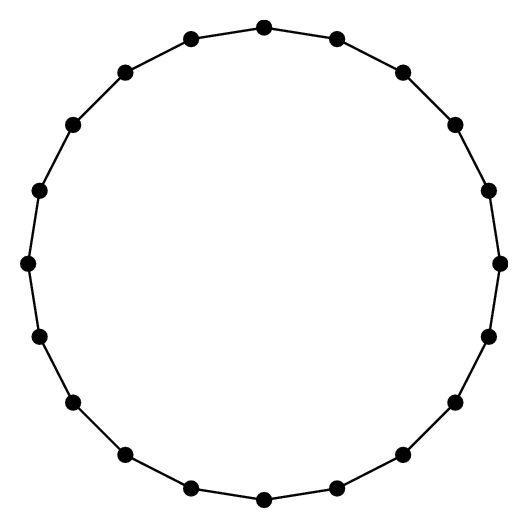
\includegraphics[width=8cm]{../Figure/Q1/ring.jpg} 
 \end{figure}


\lr{\begin{table}[H]
		\caption{Parameter of ACO}
		\vspace{0.5cm}
		\centering
		\begin{tabular}{|c|c|c|}
			\hline
			\lr{Value} & \lr{Parameter}\\
			\hline
			20 & \lr{Number of Particles}\\
			\hline
			2 & $C_1$\\
			2 & $C_2$\\
			0.5 & $w$\\
			\hline
		\end{tabular}
		\label{tab:PSO_par}
\end{table}}

 \begin{figure}[H]
	\caption{نمودار همگرایی الگوریتم \lr{PSO} تابع شماره یک ($D=10$) برای ۱۰۰۰ تکرار } 
	\centering 
	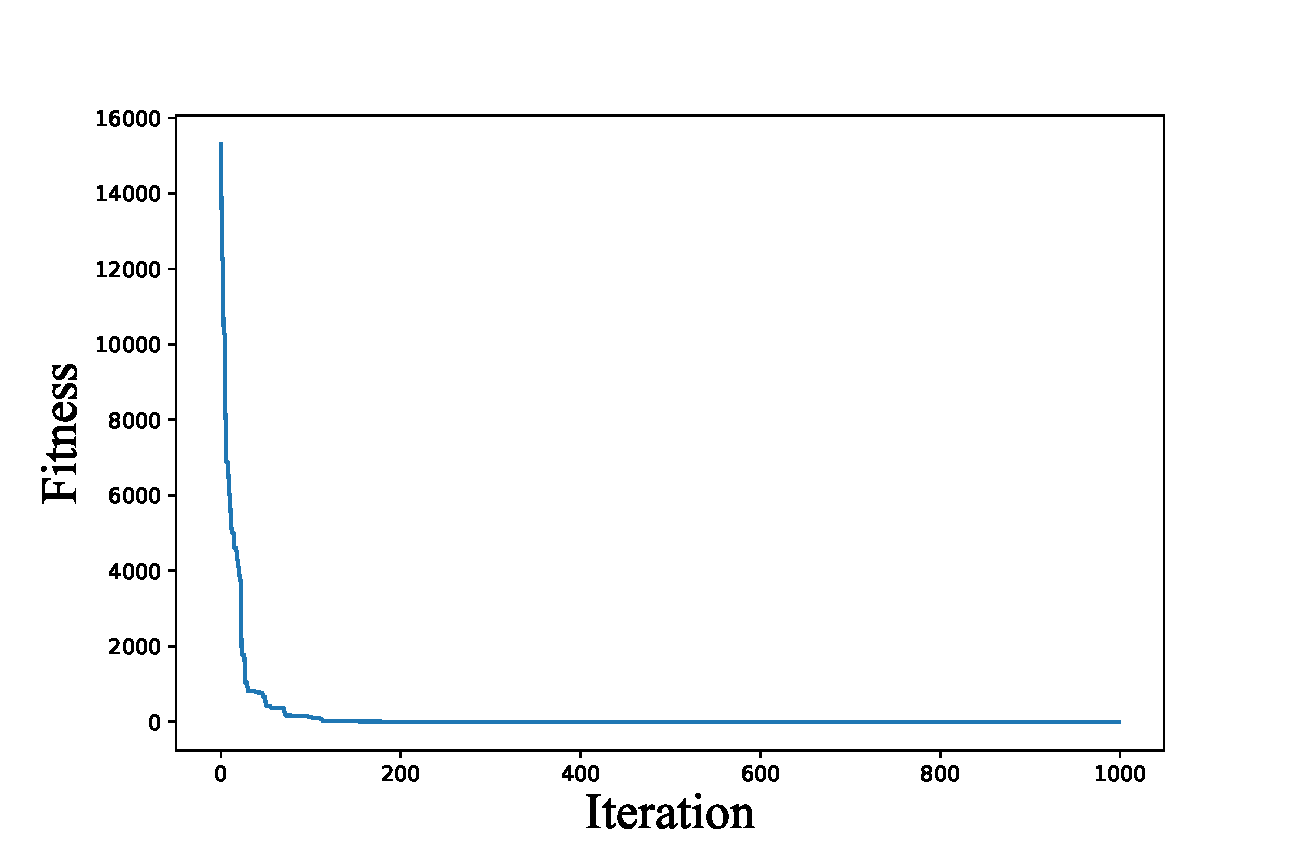
\includegraphics[width=16cm]{../Figure/Q1/PSO_convergence_curve} 
\end{figure}

 \begin{figure}[H]
	\caption{نمودار \lr{inertia weight} الگوریتم \lr{PSO} تابع شماره یک ($D=10$) برای ۱۰۰۰ تکرار } 
	\centering 
	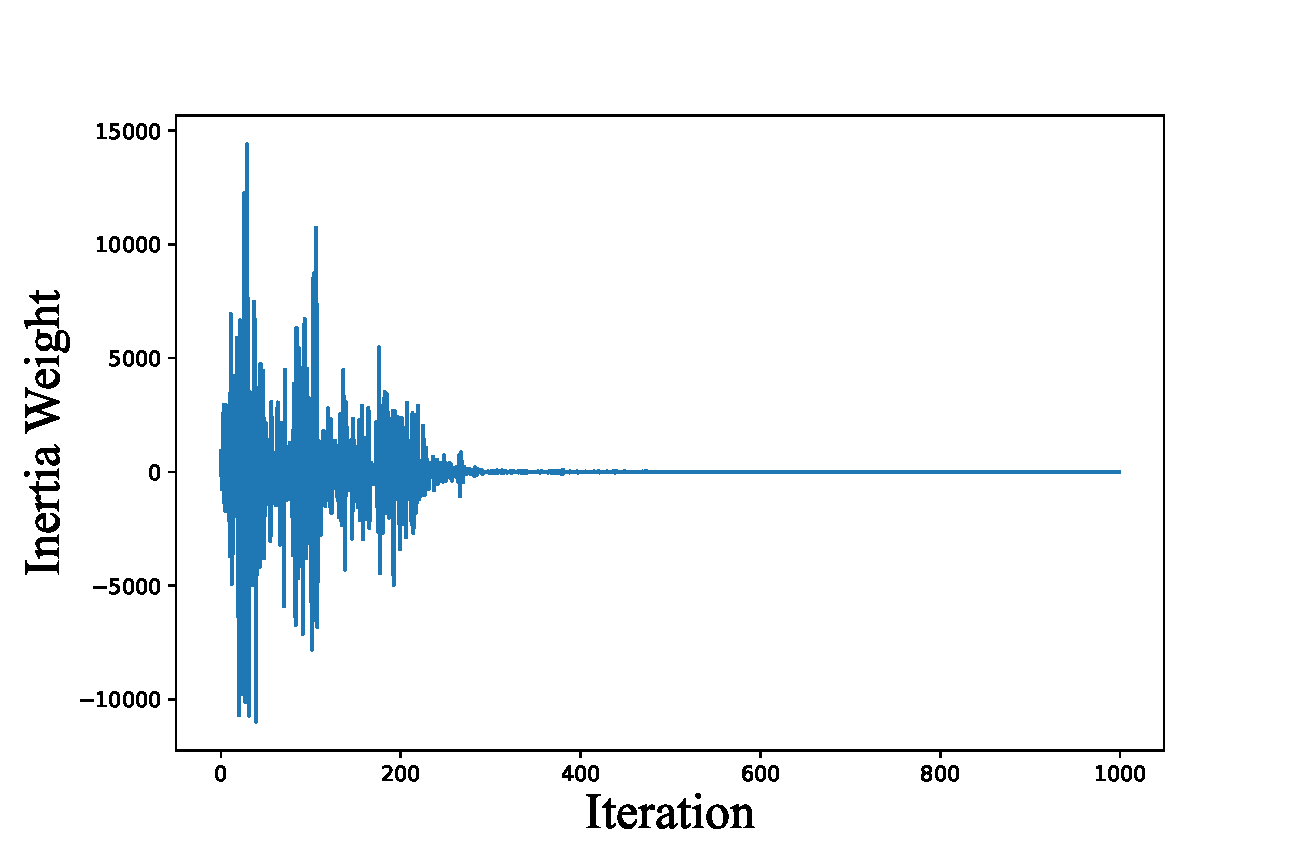
\includegraphics[width=16cm]{../Figure/Q1/PSO_inertia_weight} 
\end{figure}

 \begin{figure}[H]
	\caption{نمودار همگرایی الگوریتم \lr{PSO} تابع شماره دو ($D=10$) برای ۱۰۰۰ تکرار } 
	\centering 
	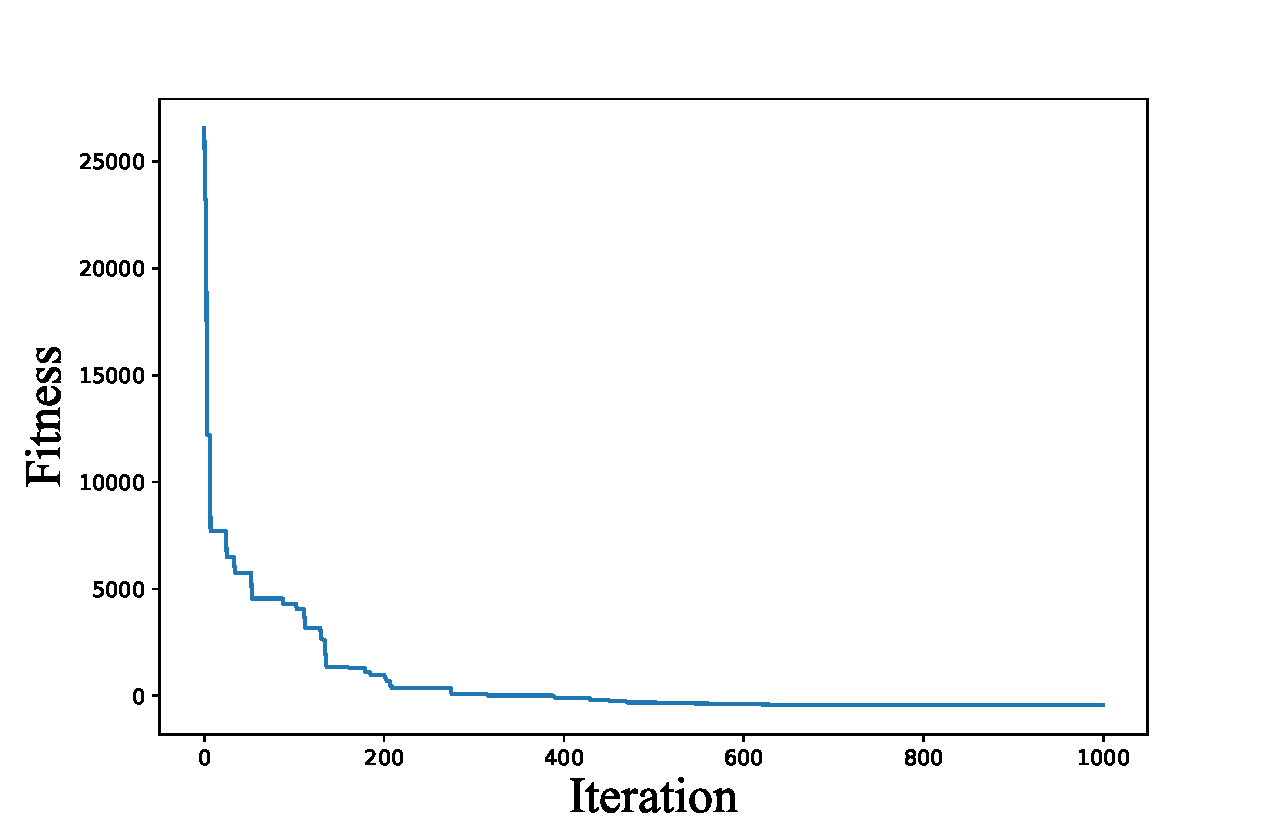
\includegraphics[width=16cm]{../Figure/Q1/PSO_II_convergence_curve} 
\end{figure}

\begin{figure}[H]
	\caption{نمودار \lr{inertia weight} الگوریتم \lr{PSO} تابع شماره دو ($D=10$) برای ۱۰۰۰ تکرار } 
	\centering 
	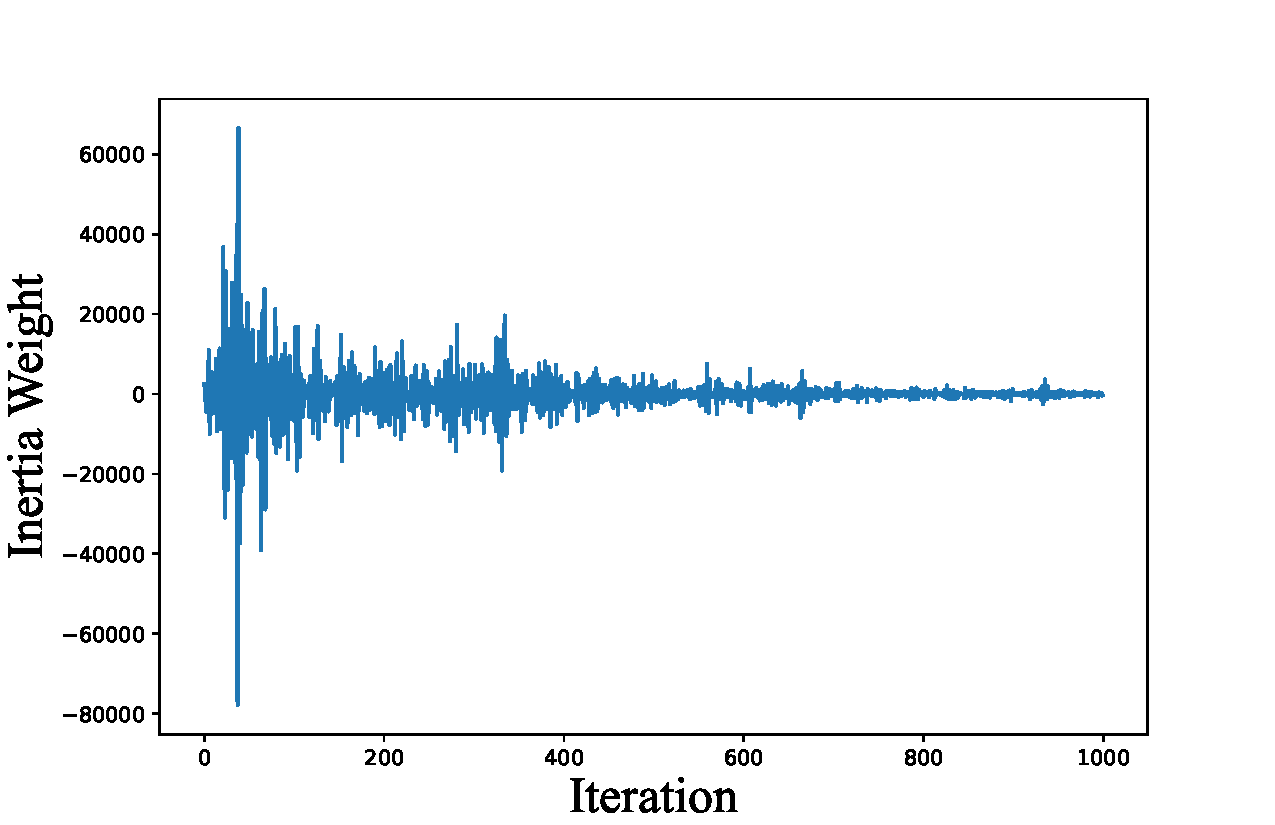
\includegraphics[width=16cm]{../Figure/Q1/PSO_II_inertia_weight} 
\end{figure}

به علت اینکه تابع شماره دو دارای نویز است، پس، 
\lr{inertia weight}
آن نیز دارای نویز است.

	\lr{\begin{table}[H]
		\caption{Values Achieved with PSO algorithm for Problems 1 and 2 (D=10)}
		\vspace{0.5cm}
		\centering
		\begin{tabular}{|c|c|c|c|}
			\hline
			\lr{Problem 2} & \lr{Problem 1}  &  \multicolumn{2}{ |c| }{FES/Problem} \\
			\hline
			-449.99999999999955 & -449.9999787052277 & \lr{$1^{th}$(Best)} & \multirow{7}{*}{1e3}  \\
			-449.9999999983805 & -449.999853416358 & \lr{$7^{th}$} & \\
			-449.999985766405 & -449.9996680779018 & \lr{$13^{th}$(Median)} & \\
			-449.8254439788584 & -449.9992664160519 & \lr{$19^{th}$} & \\
			-61.45240223709476 & -449.9935680412684 & \lr{$25^{th}$(Worst)} & \\
			-423.450611298781 & -449.9992093850963 & \lr{Mean} & \\
			81.2593245611484 & 0.001321429062858954 & \lr{Std} & \\ \hline
			-449.99999999999966 & -450.0 & \lr{$1^{th}$(Best)} & \multirow{7}{*}{1e4}  \\
			-449.999999990536 & -450.0 & \lr{$7^{th}$} & \\
			-449.9890024477813 & -449.99999999999994 & \lr{$13^{th}$(Median)} & \\
			-429.92744443669807 & -449.99999999999994 & \lr{$19^{th}$} & \\
			4782.609097090884 & -449.99999999999983 & \lr{$25^{th}$(Worst)} & \\
			-129.8996247758574 & -450.0 & \lr{Mean} & \\
			1068.5144300632844 & 5.796914039811765e-14 & \lr{Std} & \\ \hline
			-450.0 & -450.0 & \lr{$1^{th}$(Best)} & \multirow{7}{*}{1e5}  \\
			-450.0 & -450.0 & \lr{$7^{th}$} & \\
			-450.0 & -450.0 & \lr{$13^{th}$(Median)} & \\
			-449.99999999999994 & -449.99999999999994 & \lr{$19^{th}$} & \\
			-449.99999999999994 & -449.99999999999994 & \lr{$25^{th}$(Worst)} & \\
			-450.0 & -450.0 & \lr{Mean} & \\
			3.215549355384371e-14 & 3.215549355384371e-14 & \lr{Std} & \\ \hline
		\end{tabular}
\end{table}}

	\lr{\begin{table}[H]
		\caption{Values Achieved with PSO algorithm for Problems 1 and 2 (D=30)}
		\vspace{0.5cm}
		\centering
		\begin{tabular}{|c|c|c|c|}
			\hline
			\lr{Problem 2} & \lr{Problem 1}  &  \multicolumn{2}{ |c| }{FES/Problem} \\
			\hline
-449.99999999939354 & -449.99998619166854 & \lr{$1^{th}$(Best)} & \multirow{7}{*}{1e3}  \\
40420.10955750148 & -449.9998718525022 & \lr{$7^{th}$} & \\
56691.59162357271 & -449.9998195592621 & \lr{$13^{th}$(Median)} & \\
79561.30101108812 & -449.99942177358423 & \lr{$19^{th}$} & \\
123160.65222491047 & -449.9985720932928 & \lr{$25^{th}$(Worst)} & \\
58183.77085117807 & -449.99962402843727 & \lr{Mean} & \\
30723.13488958691 & 0.0003711894716529072 & \lr{Std} & \\ \hline
23595.40655734655 & -450.0 & \lr{$1^{th}$(Best)} & \multirow{7}{*}{1e4}  \\
33363.7352014709 & -450.0 & \lr{$7^{th}$} & \\
47183.89788197362 & -449.99999999999994 & \lr{$13^{th}$(Median)} & \\
60886.23378363138 & -449.99999999999994 & \lr{$19^{th}$} & \\
103569.85779628623 & -449.99999999999994 & \lr{$25^{th}$(Worst)} & \\
49939.64569103153 & -450.0 & \lr{Mean} & \\
21155.063674898593 & 4.5474735088646414e-14 & \lr{Std} & \\ \hline
42625.903518764586 & -450.0 & \lr{$1^{th}$(Best)} & \multirow{7}{*}{1e5}  \\
76377.64509731466 & -450.0 & \lr{$7^{th}$} & \\
98728.87253737042 & -450.0 & \lr{$13^{th}$(Median)} & \\
128860.87687077752 & -449.99999999999994 & \lr{$19^{th}$} & \\
179366.99419346155 & -449.99999999999994 & \lr{$25^{th}$(Worst)} & \\
99025.05071090581 & -450.0 & \lr{Mean} & \\
34041.49636204158 & 3.215549355384371e-14 & \lr{Std} & \\ \hline
		\end{tabular}
\end{table}}

	\lr{\begin{table}[H]
		\caption{Values Achieved with PSO algorithm for Problems 1 and 2 (D=50)}
		\vspace{0.5cm}
		\centering
		\begin{tabular}{|c|c|c|c|}
			\hline
			\lr{Problem 2} & \lr{Problem 1}  &  \multicolumn{2}{ |c| }{FES/Problem} \\
			\hline
18439.04388319432 & -449.99998100894874 & \lr{$1^{th}$(Best)} & \multirow{7}{*}{1e3}  \\
44613.926387444895 & -449.9999238343942 & \lr{$7^{th}$} & \\
69394.46049754831 & -449.9998536654368 & \lr{$13^{th}$(Median)} & \\
96414.65498879585 & -449.9996903867559 & \lr{$19^{th}$} & \\
153348.96108922383 & -449.99863762582254 & \lr{$25^{th}$(Worst)} & \\
69754.01098699088 & -449.99973406754907 & \lr{Mean} & \\
37537.44745190397 & 0.0003002225766163943 & \lr{Std} & \\ \hline
123434.7542796172 & -450.0 & \lr{$1^{th}$(Best)} & \multirow{7}{*}{1e4}  \\
161688.4767345813 & -450.0 & \lr{$7^{th}$} & \\
196405.68546559024 & -449.99999999999994 & \lr{$13^{th}$(Median)} & \\
260789.9331202219 & -449.99999999999994 & \lr{$19^{th}$} & \\
380963.02282124246 & -449.99999999999994 & \lr{$25^{th}$(Worst)} & \\
215538.32784349122 & -450.0 & \lr{Mean} & \\
73059.88366852782 & 4.5474735088646414e-14 & \lr{Std} & \\ \hline
		\end{tabular}
\end{table}}